\documentclass[a4paper,10pt]{article}
\usepackage[utf8]{inputenc}
\usepackage{hyperref}
\usepackage{graphicx}
\usepackage{amssymb}
\usepackage{amsmath}
\usepackage[margin=0.7in]{geometry}

%opening
\title{Building a Granular Dataset of UK Companies}
\author{Alfred Holmes}
\date{September 2018}
\begin{document}


\maketitle
\begin{abstract}Given employment size distributions of enterprises by location and industry individually, and granular company registry data, it is possible to produce a detailed granular dataset of UK companies (containing the age, employment size, number of branches and location through time of each company) by assuming a simple growth model. To study the accuracy of the size assignments, it is possible to develop simulations to test the ability of the assignment methods to reproduce model parameters. 
\end{abstract}
 
\section{Introduction}
Contemporary economic modeling requires detailed granular data. Typically highly granular data is not available due to difficulties collecting such data or privacy issues in releasing the information. In the case of UK companies data, an ideal dataset would contain the size (employment and turnover) along with location through time and branches of the companies operating in the UK. The UK Companies House service provides basic company data on active companies, which can, as detailed in this report, be used to provide the backbone of a dataset. The entities registered on companies house are used for legal purposes for the government to track companies operating in the UK, and this legal information is freely available and so does not contain useful data such as the location of branches, number of employees and turnover information\footnote{For large companies, they are required to publish turnover information, but this is not in a machine readable format}. The ONS does produce detailed agglomerated data, giving size distributions by location and company type, but these distributions do not give data about different companies. Using these distributions, the companies house data and simple models of company growth, it is possible to assign sizes to the companies house entities to compile a detailed granular dataset of UK companies and their branches. This report explains the process of producing that dataset and its evaluation using other ONS data.  

\subsection{Data}
\subsubsection{Companies House}
Companies House release a monthly snapshot of basic data (Company ID, Address, SIC Code) of active companies on their service. This data is only available for the current month - they do offer the purchase of a DVD with historic data - but previous months (approximately one for each year) can be accessed through websites which archive the internet. There is also an API that can be used to get more detailed data (address changes, number of registered people of significant control) which has been used in this study to get company migrations. These migrations can be inferred by changes in location between two snapshots, but in using the API the exact date of the change of location is known. The API is also required to get the correct date of death of companies, since the monthly snapshots only contain active companies.

\subsubsection{ONS}
The office of national statistics provide a large range of agglomerated statistics. For use assigning values to companies, it's useful to have one statistic broken down in multiple ways. For example in the business activity, size and location tables, ONS release the number of enterprises with 0-4 employees in each local authority as well as the number of enterprises with 0-4 employees with a certain SIC code. This allows properties to be assigned to companies in a more accurate way since the extra data reduces the size of the solution space of the problem.

\subsection{Description of Terms}
Since there are different types of entities in each of the datasets, it is worth defining terms to improve the clarity and precision of descriptions.
\begin{itemize}
 \item Company - an entity registered on Companies House. In June 2017 there were 3.1 million registered companies in the UK. 
 \item Enterprise - a business that is reported by ONS. We assume that an enterprise is a collection of companies. In 2017 the ONS reported 2.7 million enterprises.
 \item Local Unit - a site where an enterprise operates, e.g. a branch of a large supermarket chain or the only location from which a small firm operates.
 \item Local Authority - a connected area of land the UK governed by a council. At the time of writing, local authorities have a population of 170 000 people and 7 000 enterprises on average. There are 391 local authorities in the UK.
\end{itemize}
\section{Matching Enterprises and Companies}


\subsection{Assigning Companies to Enterprises}
Each enterprise is made up of one or more companies. A quick way of choosing the groups of companies that make up an enterprise is to match the addresses. The motivation for this is that enterprises may register companies to handle a fraction of their total business, for example on companies house TESCO is a registered company as well as TESCO Holdings, but in making the assumption that TESCO will be reported as one enterprise, it makes sense to omit the TESCO Holdings. This results in a more linear relationship between the number of companies and enterprises in each local authority.
\begin{figure}[!ht]
 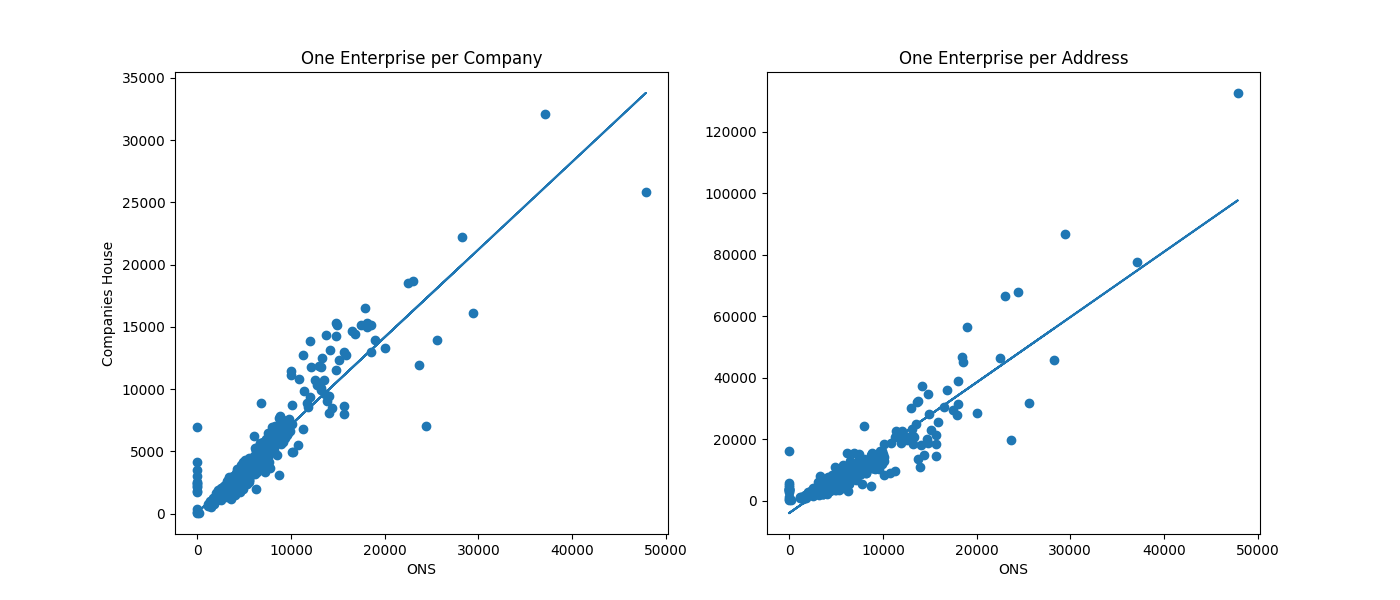
\includegraphics[width=\textwidth]{graphics/filtered_addresses}
 \caption{Improvements in grouping enterprises by addresses}
\end{figure}

After assigning companies to enterprises in this way there is a large number of enterprises missing. This could be because some companies have exempted themselves from reporting to companies house, or an issue with grouping the companies by address. In total for 2017, after the companies have been grouped together there are about 1.6 times as many enterprises as company groups. An effective way to get around this is to assign ratios by SIC code and assume that the enterprises that aren't registered are a representative sample of all the enterprises. We then make the further assumption that this grouping of companies in each SIC code is a representative sample, that is, the distribution of ages and locations by SIC code of the enterprises is the same as the companies groupings. In applying these ratios, the companies house data makes a good prediction for the number of companies in each local authority (figure \ref{predicting number of enterprises}).
\begin{figure}[!ht]
 \begin{center}
 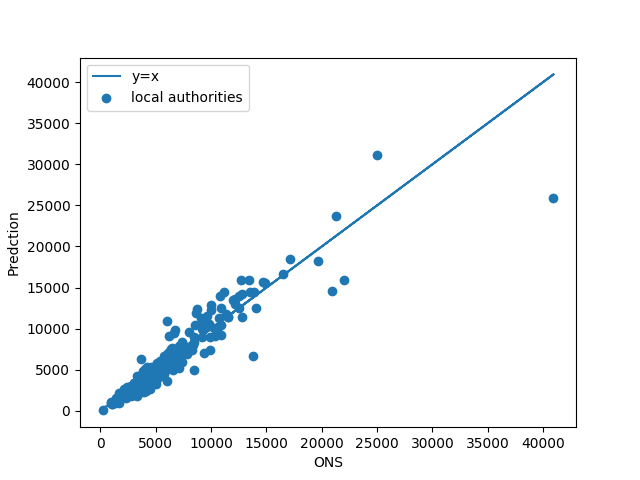
\includegraphics[width=300px]{graphics/la_enterprise_predictions_with_ch}
 \end{center}
 \caption{Predicting the number of enterprises using SIC ratios}
 \label{predicting number of enterprises}
\end{figure}


\subsection{Enterprises Size Distributions}
\label{enterprise_sizes}
The ONS tables of size by SIC code and location are given with the sizes in bands - so the number of companies in a certain SIC code with number of employees between 50 and 100 is given for example. It is possible to fit a log normal distribution to these size bands\footnote{see appendix, section \ref{ONS size dist parameter fitting}}. Since there is quite limited data due to the size bands, it is difficult to test whether these distributions are a good fit, but the appearance of log normal distributions in company size distributions is well documented. There are also other sources of data to test these distributions since the ONS releases the total employment by local authority and as the total number of companies and size distribution per local authority is known, employment predictions can be made of the total private sector employment.


\subsubsection{Dependence on Location and SIC Code}
It is possible to test whether the main determinant of a enterprise's size is it's SIC code, location or a combination by, for example, seeing whether fitting the size distribution for the location and assigning sizes to companies from that distribution predicts the other distribution. In general this is not the case, suggesting that the factors effecting an enterprise's growth depends on its location and SIC code.


\section{Models for company growth}

In order to make the solution space of size assignments smaller, it makes sense to assume a growth model for companies and fit parameters. This has two benefits: allowing the knowledge of enterprise ages be used to assign company sizes and giving the enterprises sizes a realistic time evolution.  
\subsection{Gibrat Model}
This is a simple model from which the main model is based. Suppose that that the size of a company with age $i$ is given by
\begin{equation}
 X_i = \prod_{j=1}^{i}(1 + \epsilon_j)
 \label{company_size}
\end{equation}
where $\epsilon_i \sim \mathcal{N}(\alpha, \beta^2)$. This means that if $X$ represents the size of an enterprise picked at random then
\begin{equation}
 X = \sum_{i}\mathbf{1}_{Zi}X_i
 \label{overall_dist}
\end{equation}
where $\mathbf{1}$ is an indicator function and $Z$ is a random variable such that $\mathbb{P}(Z = i) = \frac{n_i}{N}$ where $N$ is the number of enterprises with the given SIC and local authority and $n_i$ is the number of companies with age $i$. If the distribution of $X$ is known, the parameters $\alpha$ and $\beta$ can be calculated by matching $\mathbb{E}(X)$ and $\mathrm{Var}(X)$\footnote{The parameter fitting for this model is very similar to the parameter fitting in section \ref{model parameter fitting}}. Unfortunately, if it is assumed that all companies in the UK evolve in this way with the same parameters it is only possible to match the expectation as the variance in all the companies is too high with $\beta = 0$ due to the underlying variation in ages. The same is generally true for the size distributions by local authority and SIC code. It is possible that the assumption that the size of each company starts at 1 is causing these issues, but without data on the initial state of companies, is it not possible to come up with a better starting size distribution.
\subsection{Adapted Gibrat Model}
The problem with the previous model is that with the given ages from the companies and the fitted means, the variance is too high with no variance in the growth process. To get around this, suppose that the number of employees  $X_i^s$ belonging to an enterprise registered in local authority $l$, with SIC code $s$ that is $i$ months old has size:
\begin{equation}
 X_i = \prod_{j = 1}^i(1 + \alpha_j + \beta_j)
 \label{2 parameter model}
\end{equation}
Where $\alpha_j \sim \mathcal{N}(\mu_l, \sigma^2_l)$ and $\beta_j \sim \mathcal{N}(\nu_s, \tau^2_s)$. So $\alpha$ is a property of the local authority and $\beta$ is a property of the SIC code. 
Dropping the subscripts, we assume that $\mu$, $\nu$, $\sigma$, and $\tau$ are suitably small such that $\log(1 + \alpha + \beta)$ is approximately normally distributed. By the log normal sum approximation\footnote{See appendix, section \ref{Log Normal Sum Approximation}} this implies that the national size distribution of companies is log normally distributed, as well as the cross sections by SIC code and location, as seen in the data and previous work.
\subsubsection{Parameter Fitting}
\label{model parameter fitting}
Assuming this model, it is possible to fit the parameters by matching the mean and variance of the observed size distributions. Here we will focus on using the local authority distributions, but the process is the same for the SIC codes.
\\\\ Let $X$ be a random variable representing the size of a firm picked at random from a local authority $l$. After fitting a log normal distribution to the ONS data\footnote{See appendix, section \ref{ONS size dist parameter fitting}}, the mean and variance of the observed size distributions are known. From (\ref{2 parameter model}):
\begin{align}
 X = \sum_{s \in S} \sum_{i \in A}\mathbf{1}_{Z(s,i)}X_i^s
\end{align}
where $\mathbf{1}$ is an indicator function, and $Z$ is a random variable which represents drawing a random SIC code and age. This means that, if $N$ is the total number of companies, and $n_{si}$ is the number of companies, age $i$ with SIC code $s$ in the local authority, then:
\begin{align}
 \label{expectation of la size}
 \mathbb{E}(X) &= \frac{1}{N}\sum_{s \in S}\sum_{i \in A}n_{si}\mathbb{E}(X_i^s)\\
 &= \frac{1}{N}\sum_{s \in S}\sum_{i \in A}n_{si}(1 + \mu_l + \nu_s)^i
\end{align}
and 
\begin{align}
 \label{variance of la size}
 \mathrm{Var}(X) &= \sum_{s, t \in S}\sum_{i, j \in A}\mathrm{Cov}(\mathbf{1}_{Z(s, i)}X_i^s, \mathbf{1}_{Z(t, j)}X_j^t)\\
 &= \sum_{s, t \in S}\sum_{i, j \in A}\delta_{st}\delta_{ij}\frac{n_{si}}{N}\left(\sigma_l^2 + \tau_s^2 + (1 + \mu_l + \nu_s)^2\right)^i - \frac{n_{si}n_{tj}}{N^2}(1 + \mu_l + \nu_s)^i(1 + \mu_l + \nu_t)^j
 \label{variance of la size 2nd}
\end{align}
. From (\ref{expectation of la size}) the model provides an equation for each local authority, and similarly for each SIC code, so it is possible to calculate $\mu_l$ and $\nu_s$ for all $l$ and $s$ and in the same way (\ref{variance of la size}) provides equations for $\sigma_l$ and $\tau_s$. Luckily the calculation of the change in the total variance with changing the parameters $\sigma$ and $\tau$ scales like $N^2$ not $N^4$ since the second term in the summand of ($\ref{variance of la size 2nd}$) can be calculated once beforehand, so numerical methods can be used with the whole dataset.

\section{Local Units}
In order to measure useful quantities, like employment, it is important to have data on the local units. There is a strong linear relationship between the number of local units and the number of enterprises in each local authority. The interpretation of this is that in areas with more registered companies (and therefore more enterprises) there is more economic activity which results in more local units being present, not that on average a company has $\alpha$ local units in the local authority that it is registered. Using this approach the number of local units can be calculated from companies data.
\\ Once the number of local units is known, there is another assignment problem of the local units to the enterprises. To perform this assignment we make the assumptions:
\begin{enumerate}
 \item Each enterprise has at least one local in the same local authority as the enterprise. This local unit employs at most as many people as the enterprise.
 \item 
\end{enumerate}

\section{Results}
\subsection{Dataset}
\subsection{Total Employment}
\subsection{Employment Migration}

\section{Appendix}
\subsection{Size Bands and Log Normal parameter fitting}
\label{ONS size dist parameter fitting}
The ONS typically release enterprise and local unit size data in bands, so they give the number of companies, $n_i$ with size $x \in [a_i, a_{i+1})$ by some other parameter (SIC code or location). Assuming a log normal distribution where the size X of a company is such that $\log X \sim \mathcal{N}(\mu, \sigma^2)$, $\mu$ and $\sigma$ can be calculated by maximising the log likelihood, given by
\begin{equation}
 l(\mu, \sigma) = \sum_i n_i \log \left( \Phi \left( \frac{\log a_{i + 1} - \mu}{\sigma} \right) - \Phi \left( \frac{\log a_{i} - \mu}{\sigma} \right) \right)
\end{equation}
since $\mathbb{P}(a_i < X < a_{i + 1}) = \mathbb{P}(\log a_i < \log X < \log a_{i + 1}) = \Phi \left( \frac{\log a_{i + 1} - \mu}{\sigma} \right) - \Phi \left( \frac{\log a_{i} - \mu}{\sigma} \right)$. \\
For the employment size distributions of enterprises and local units the the fitted parameters predict the ratios $\frac{n_i}{N}$ well and in the case of local authorities the distributions predict the total employment well so it is perhaps reasonable to assume that the actual distribution is log normal. Whether it is possible for other distributions (Yule or other fat tailed distributions) to reproduce these results is something worth testing, but for the purposes of predicting enterprise and local unit sizes, the log normal distribution seems to work well.

\subsection{Log Normal Sum Approximation}
\label{Log Normal Sum Approximation}
Given an indexed set of random variables $\{X_i\}$ such that $\log X_i \sim \mathcal{N}(\mu_i, {\sigma_i}^2)$ an important question for this study is whether the random variable $X = \sum_i\mathbf{1}_{Zi}X_i$ has a distribution that is approximately log normal, and whether there exist non trivial requirements of the distribution ${(\mu_i, \sigma_i)}$ given the distribution of $Z$ for $X$ to be log normally distributed\footnote{A trivial example is that $\forall i, \ (\mu_i, \sigma_i) = (\mu, \sigma)$, so $X = kX_i$ and is therefore log normally distributed.}. If this were the case then the fact that there is a conservation of the log normal distributions and that the distribution of $Z$ is known, then a more accurate prediction of ${(\mu_i, \sigma_i)}$ could be calculated to get a better prediction of company size.
Running simulations with the given data, to make sure that the parameter choice is relevant, results in $X$ being approximately log normally distributed for both the local authority distributions and SIC distributions. %TODO: expand and test this claim, hopefully say something interesing

\subsection{Adapted Gibrat Model}
The problem with the previous model is that with the given ages from the companies and the fitted means, the variance is too high with no variance in the growth process. To get around this, suppose that the number of employees  $X_i^s$ belonging to an enterprise registered in local authority $l$, with SIC code $s$ that is $i$ months old has size:
\begin{equation}
 X_i^s = \prod_{j = 1}^i(1 + \alpha_j + \beta_j)
\end{equation}
Where $\alpha_j \sim \mathcal{N}(\mu_l, \sigma^2_l)$ and $\beta_j \sim \mathcal{N}(\nu_s, \tau^2_s)$. So $\alpha$ is a property of the local authority and $\beta$ is a property of the SIC code. 
Dropping the subscripts, we assume that $\mu$, $\nu$, $\sigma$, and $\tau$ are suitably small such that $\log(1 + \alpha + \beta)$ is approximately normally distributed.
\subsubsection{Parameter Fitting}
Focusing on a given local authority, $l$, which has $m_i$ enterprises each with a size $s \in [a_i, a_{i+1}), \ a_i \in \mathbb{R}^{> 0}$, we wish to find the parameters $\mu_l$ and $\sigma_l$ as well as the set of parameters $\{(\nu_s, \tau_s) \ | \ s \in \{\text{SIC codes}\}\}$ that maximise the log likelihood:
\begin{align}
 l &= \sum_jm_j\log\left(\sum_s\sum_i\frac{n_{is}}{N_l}\mathbb{P}(X_i^s \in [a_j, a_{j+1}))\right) \\
   &= \sum_j m_j \log\left(\sum_s\sum_i\frac{n_{i_s}}{N_l}\left(\Phi\left(\frac{\log a_{j+1} - i (\mu_l + \nu_s)}{\sqrt{i (\sigma^2 + \tau^2)}} \right) - \Phi\left(\frac{\log a_{j} - i (\mu_l + \nu_s)}{\sqrt{i (\sigma^2 + \tau^2)}} \right) \right) \right)
\end{align}
since $\log(1 + \alpha + \beta) \approx \alpha + \beta$ given that the parameters are sufficiently small. This parameter estimate is quite complex since all the local authorities




\end{document}
